\subsection{Kausalität}
	\begin{align*}
		P^0 > 0 ~(\text{positive Energie})
	\end{align*}
aber $\phi$ enthält $a^\dagger_{\vec{p}} \,e^{i P^0 t}$ und $a_{\vec{p}} \,e^{i P^0 t}$
\\
%Links negative Frequenzen, rechts positive Frequenzen 
$\omega_{\vec{P}} = P^0$
	\begin{align*}
		&\text{Operator von postivien Frequenzen } a_{\vec{p}} \text{ vernichtet Feld} \\
		&\text{Operator von negativen Frequenzen } a^\dagger_{\vec{p}} \text{ erzeugt Feld}
	\end{align*}
$\Rightarrow$ Insgesamt sind alle Energien positiv.

Propagator von $y$ nach $x$ ($\phi^\dagger (x) = \phi (x)$, da $\phi$ reell) 
	\begin{align*}
		\braket{0 | \phi (x) \phi(y) | 0} &= 
		\int \frac{\diff^3 p}{(2 \pi)^3} \frac{1}{2 E_p} 
		e^{- i p (x -y)} 
	\end{align*}
	\begin{align*}
		[a_{\vec{p}}, a^\dagger_{\vec{p}\,'}] &= (2 \pi)^3 \delta^{(3)} (\vec{p}- \vec{p}\,') \\
		[a_{\vec{p}}, a_{\vec{p}\,'}] &= [a^\dagger_{\vec{p}}, a^\dagger_{\vec{p}\,'}] = 0
	\end{align*}
Beispiel 1: Zeitartiger Abstand: $X^0 = Y^0 + t, \vec{X} = \vec{Y}, (X - Y)^2 > 0$
	\begin{align*}
		D (x- y) &= \frac{4 \pi}{(2 \pi)^3} \int \limits_0^\infty \diff p
		\frac{p^2}{\sqrt{p^2 + m^2}} e^{-i \sqrt{p^2 + m^2} t} \\
		&= \frac{1}{8 \pi^2} \int \limits_m^\infty \diff E \sqrt{E^2 - m^2 e^{-iEt}}
		\sim m^2 e^{-imt} \text{ für } t \rightarrow \infty
	\end{align*} 
$E = \sqrt{p^2 + m^2},~\diff E = \frac{\diff p \,p}{\sqrt{p^2 + m^2}},~ ps = \sqrt{E^2- m^2}$
\\
Beispiel 2: raumartiger Abstand $\vec{x} = \vec{y} + \vec{r}, ~ x^0 = y^0, ~(x- y)^2 = \vec{r}^2 < 0$ 
	\begin{align*}
		D(x- y) &= \int \frac{\diff^3 p}{(2 \pi)^3} \frac{1}{2 E_p} e^{- \vec{p} \vec{r}} & \int \limits_{-1}^{1} \diff \cos \theta e^{i p r \cos \theta} &= \frac{1}{i p r} (e^{ipr} - e^{-ipr}) \\
		&= \frac{1}{8 \pi^2} \int \limits_0^\infty \diff \frac{p^2}{i p r} \frac{1}{E_p} (e^{ipr} - e^{-ipr}) \\
		&= \frac{-i}{8 \pi^2 r} \int \limits_{-\infty}^\infty \diff p \frac{p}{\sqrt{p^2 +m^2}} e^{ipr}
	\end{align*}
 
	\begin{figure} [h]
		\begin{center}
			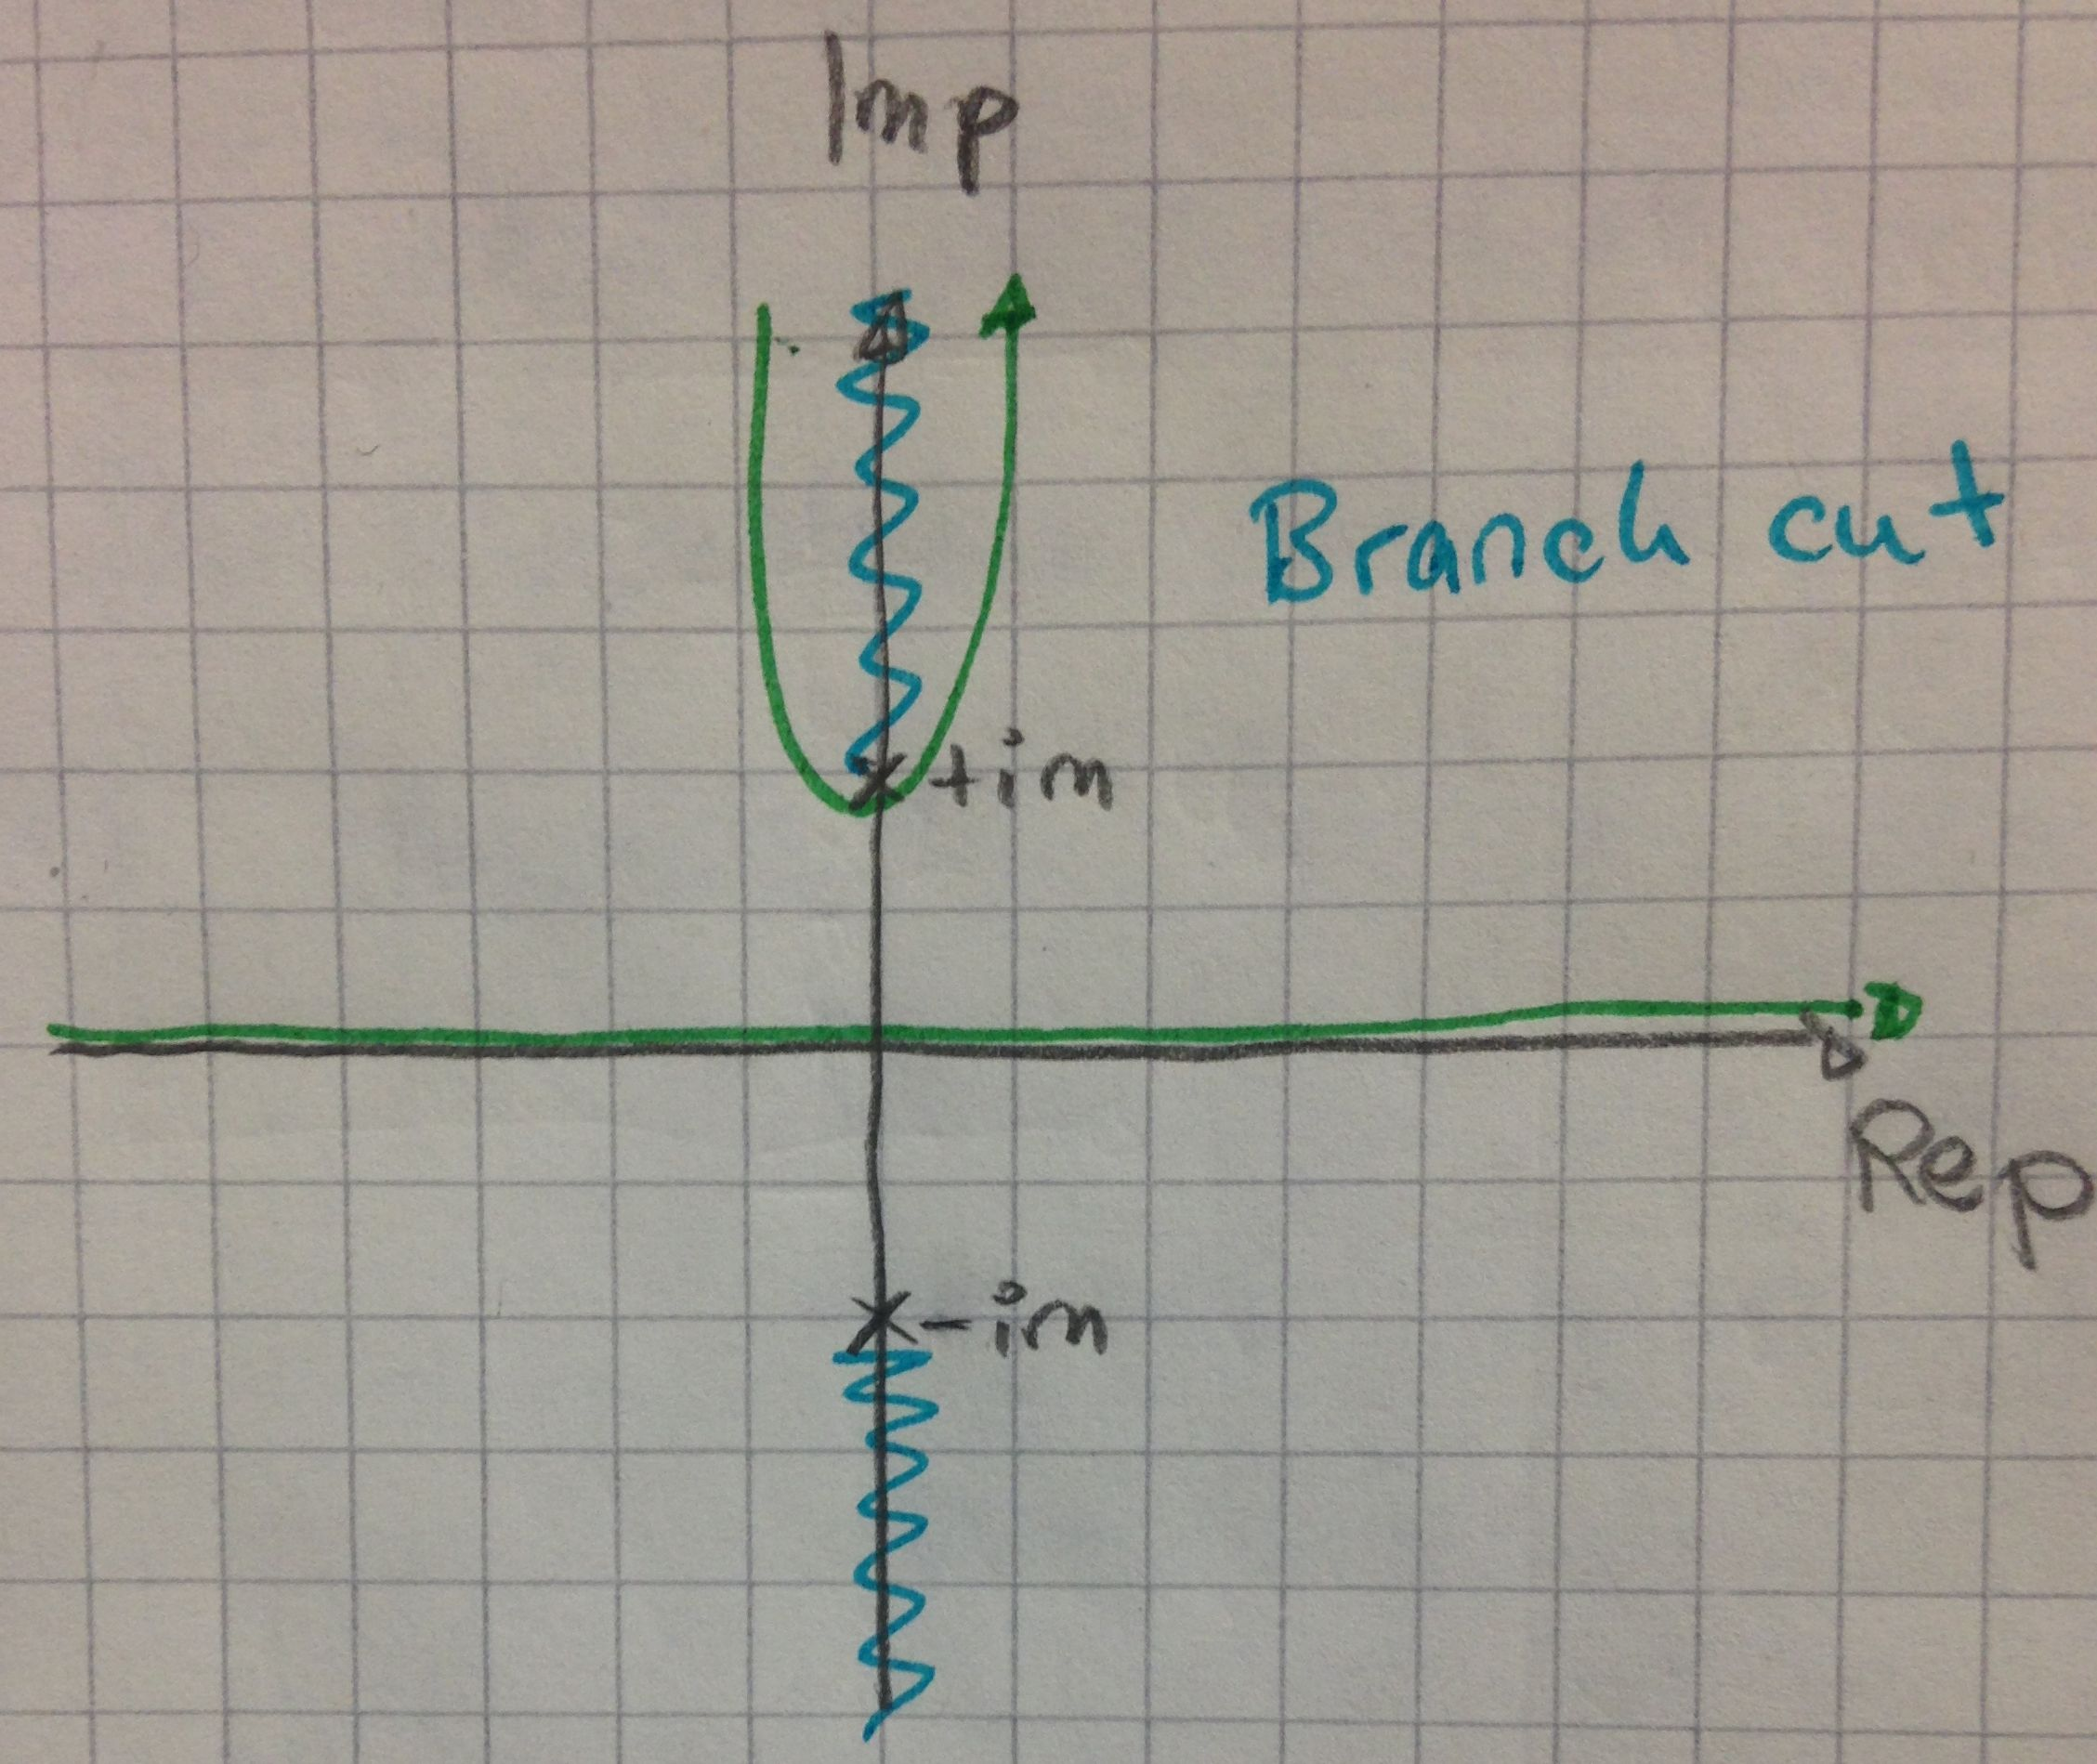
\includegraphics[width = 10cm]{Kausalitaet}
		\end{center}	
	\end{figure}
\FloatBarrier	         
	\begin{align*}
		= \frac{1}{4 \pi^2 r }\int \limits_m^\infty \diff \rho \frac{\rho}{\sqrt{\rho^2 - m^2}} e^{-\rho r} \sim m \frac{e^{-mr}}{r} (r \rightarrow \infty)
	\end{align*} 
Kann Messung des Feldes bei $x$ eine Messung bei $y$ beeinflussen. 

Hoffentlich ist $[\phi(x), \phi(y)] = 0$, für $(x- y)^2 < 0$
	\begin{align*}
		[\phi(x), \phi(y)] &= \int \frac{\diff^3 p \diff^3 p}{(2 \pi)^6} 
		\frac{1}{\sqrt{2 E_p 2E_{p\,'}}}
		\left[
			(a_{\vec{p}} \,e^{-ipx} + a^\dagger_{\vec{p}} \,e^{ipx}), 
			(a_{\vec{p}\,'} e^{-ip\,'y} + a^\dagger_{\vec{p}\,'} e^{ip\,'y})
		\right] \\
		&= \int \frac{\diff^3 p}{(2 \pi)^3} \frac{1}{2 E_p} (e^{-i p(x- y)} - e^{ip (y-x)}) = D(x - y) - D(y-x)
	\end{align*}

	\begin{figure} [h]
		\begin{center}
			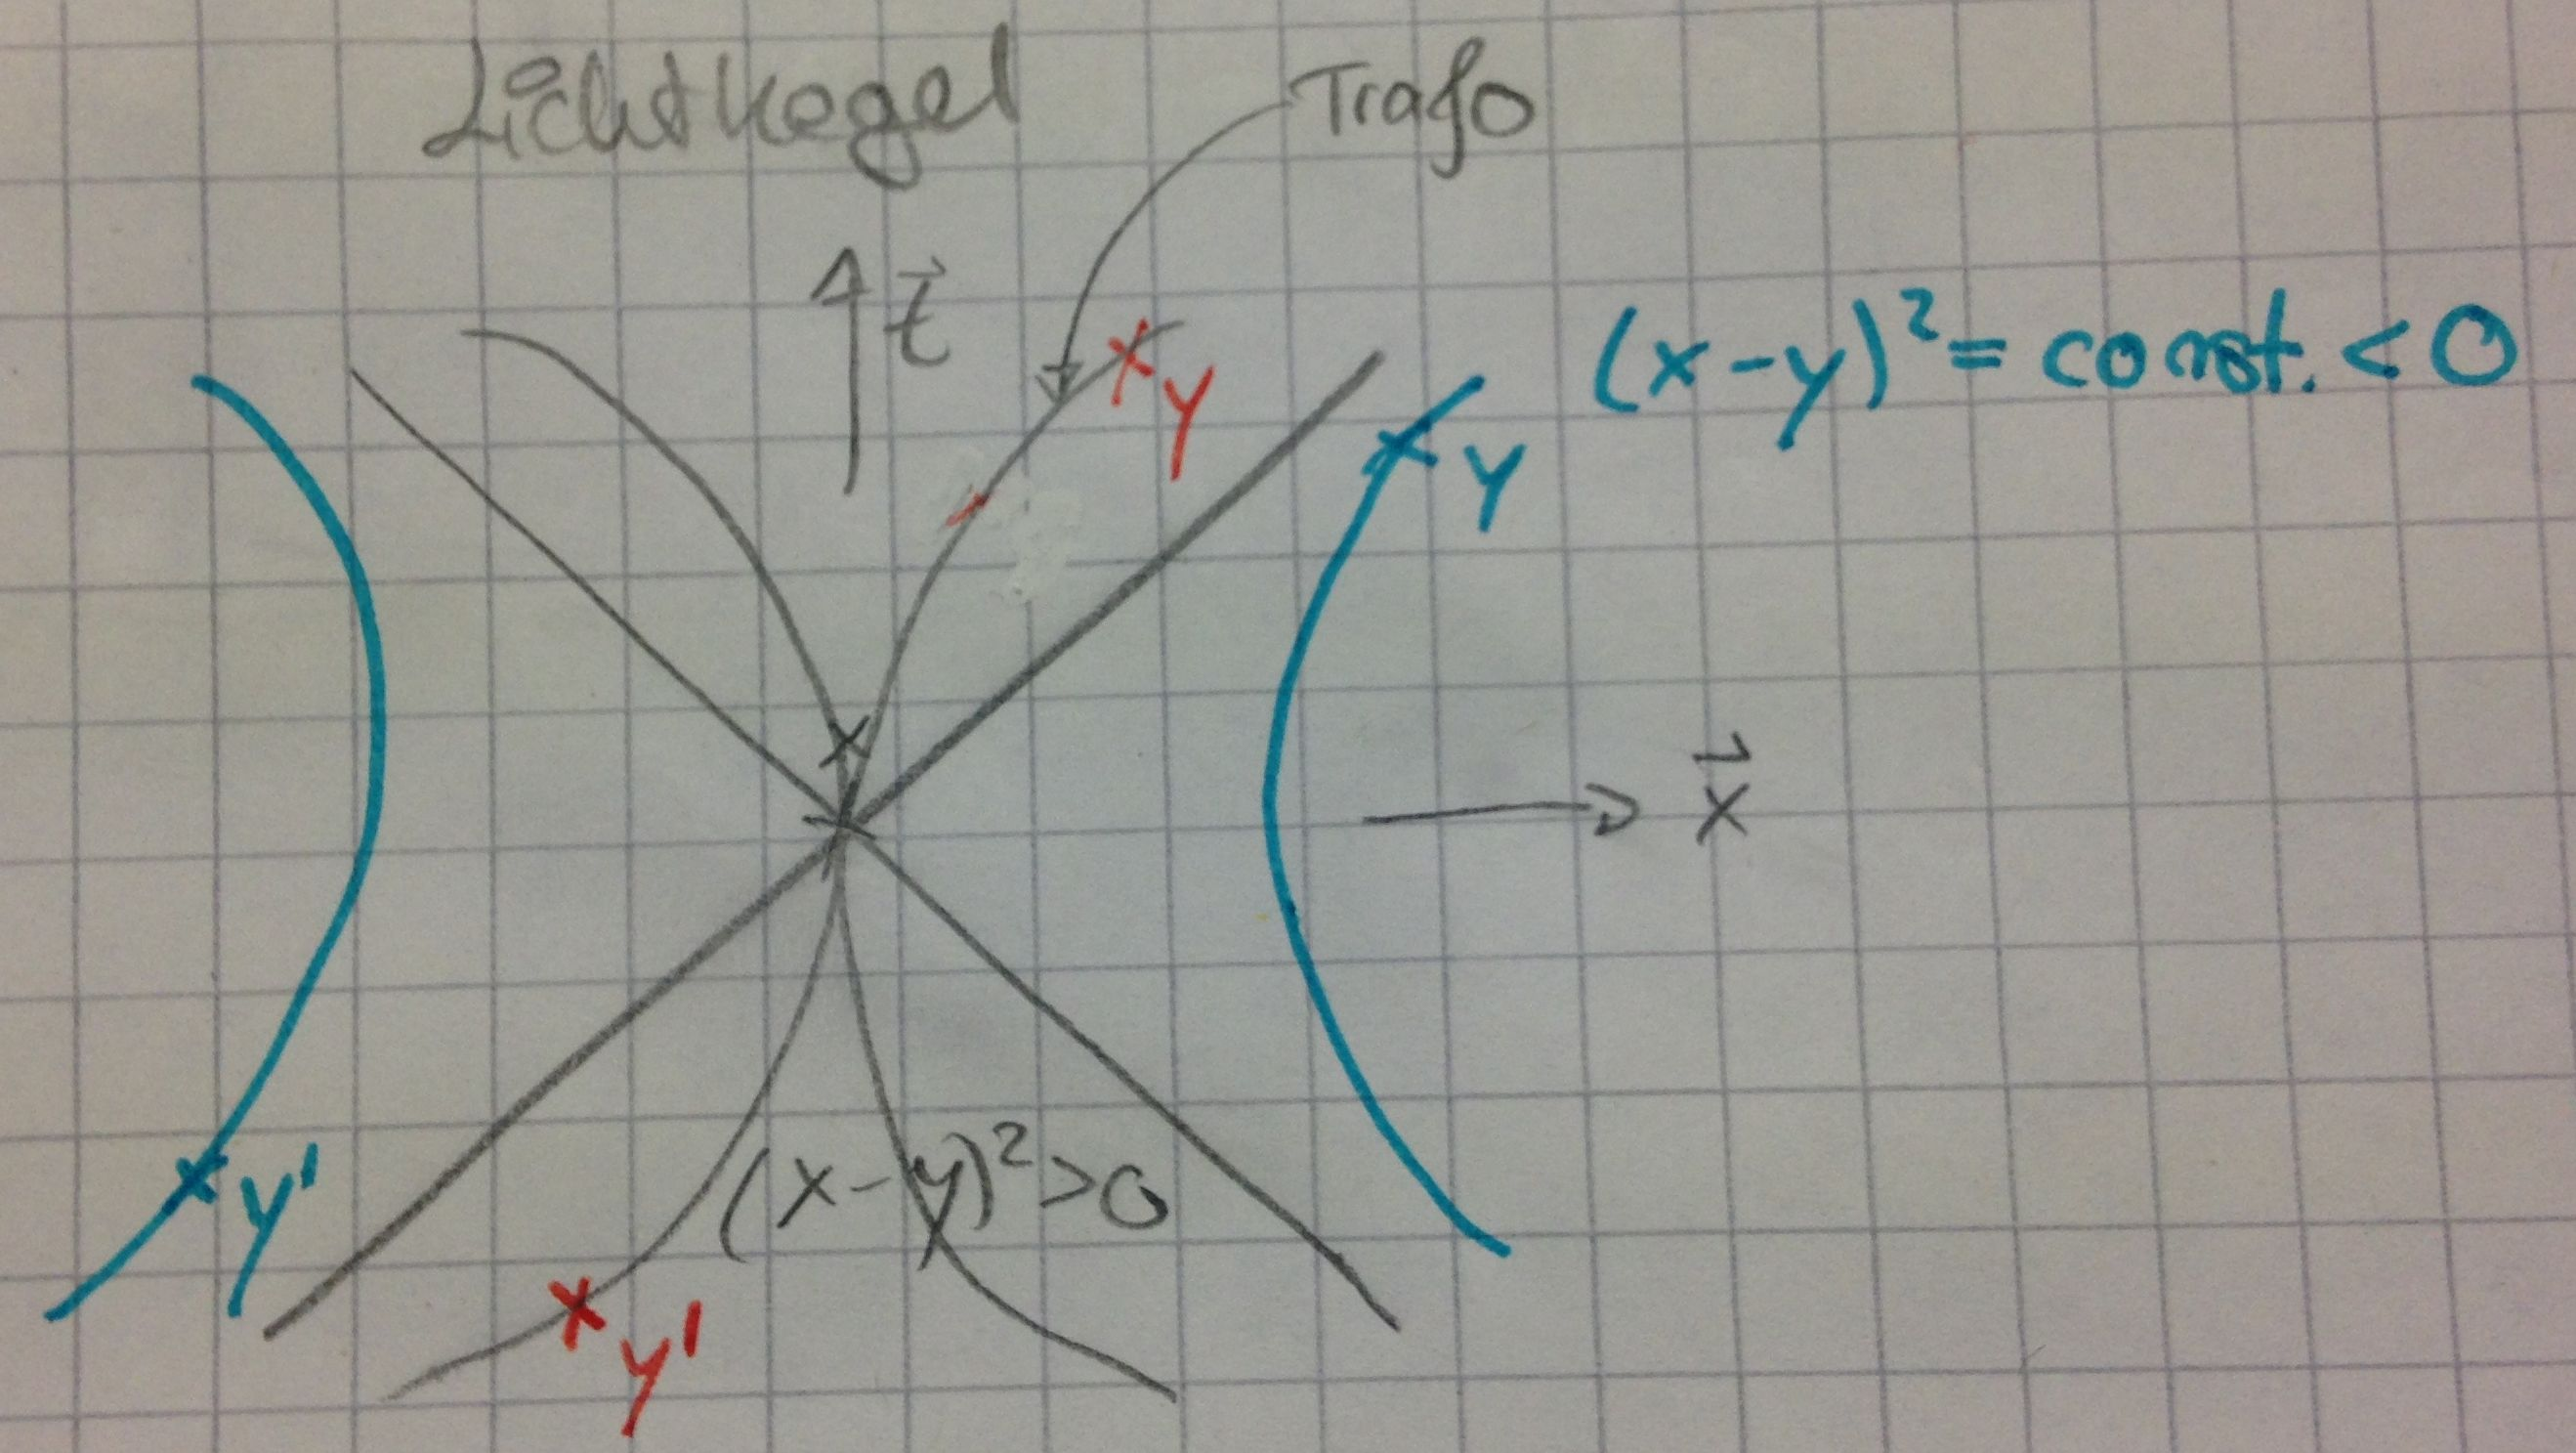
\includegraphics[width = 10cm]{Kausalitaet2}
		\end{center}	
	\end{figure}
\FloatBarrier
$(x-y) \rightarrow -(x - y)$ durch Kontinuierliche Lorenztransformation für $(x-y)^2 <0$
	\begin{align*}
		[\phi(x), \phi(y)]	= D(x - y) - D(y - x) = D(x - y) - D(-(y -x)) = 0 \checkmark 
	\end{align*} 
$(x -y)^2 \geq 0$ (nicht raumartig) $\Rightarrow$ $(x- y)$ und $-(x-y)$ sind durch keine kontinuierliche Lorentztrafo miteinander verbunden.

$\Rightarrow D(x-y) - D(y-x) \neq 0 $ im Allgemeinen

Beispiel 
	\begin{align*}
		\vec{x} = \vec{y} &\Rightarrow [\phi(x), \phi(y)]
		\underset{y^0 -x^0 \rightarrow \infty}{\longrightarrow} \sim
		\left(e^{-im(y^0 -x^0)} - e^{im (y^0 -x^0)}\right) \neq 0
	\end{align*}	
In Klein-Gordon Theorie mit komplexem Feld $\phi (x) \in \mathds{C}$ existiert elektrische Ladung $q$:

$\phi^\dagger$ erzeugt positiv geladene Teilchen/zerstört negativ geladene Teilchen

$\phi$ ~erzeugt negativ geladene Teilchen/zerstört positiv geladene Teilchen
\\
$\braket{0 | [\phi(x), \phi^\dagger(y)] | 0}$ Propagator für positiv geladenes Teilchen von $y$ nach $x$ und Propagator für negativ geladene Teilchcen von $x$ nach $y$.

reelles Klein Gordon Feld $\Rightarrow q = 0,~\phi = \phi^\dagger$ 

Konsequenz: zu jedem Teilchen existiert ein Antiteilchen gleicher Masse, aber mit negativen Quantenzahlen (hier Ladung) (Reelles K.G. Feld: Teilchen und Antiteilchen sind miteinander identisch).